\documentclass[11pt]{article}
\usepackage[margin=1in]{geometry}
\usepackage{amsmath,amssymb,amsthm}
\usepackage{graphicx}
\usepackage[hidelinks]{hyperref}

\newtheorem{theorem}{Theorem}
\newtheorem{lemma}{Lemma}
\newtheorem{remark}{Remark}

\newcommand{\T}{\mathbb T}
\newcommand{\C}{\mathbb C}
\newcommand{\calU}{\mathcal U}

\title{A counterexample to unitary lifting in operator-system ultraproducts}
\author{Run \texttt{fa\_banach\_001}, lane 17}
\date{2026-07-18}

\begin{document}
\maketitle

\section*{Source Problem}

The source is Isaac Goldbring and Martino Lupini, \emph{Model-theoretic aspects of the Gurarij operator system}, arXiv:1501.04332v3.  In Section 5, after Question 5.5 on whether the class of operator systems unitally completely order isomorphic to a C*-algebra is elementary, they ask:

\begin{quote}
Question 5.6. With the preceding notation, if \(u\) is a unitary in \(\prod_{\calU} X_i\), are there unitaries \(u_i\in X_i\) for which \(u=(u_i)^\bullet\)?
\end{quote}

Here \(X_i\) are operator systems, \(\calU\) is an ultrafilter, and ``unitary'' is meant in the Blecher-Neal operator-space sense used in the source paper: \(u\in X\) is a unitary if there is a linear complete isometry \(X\to B(H)\) sending \(u\) to the identity operator.

\begin{center}
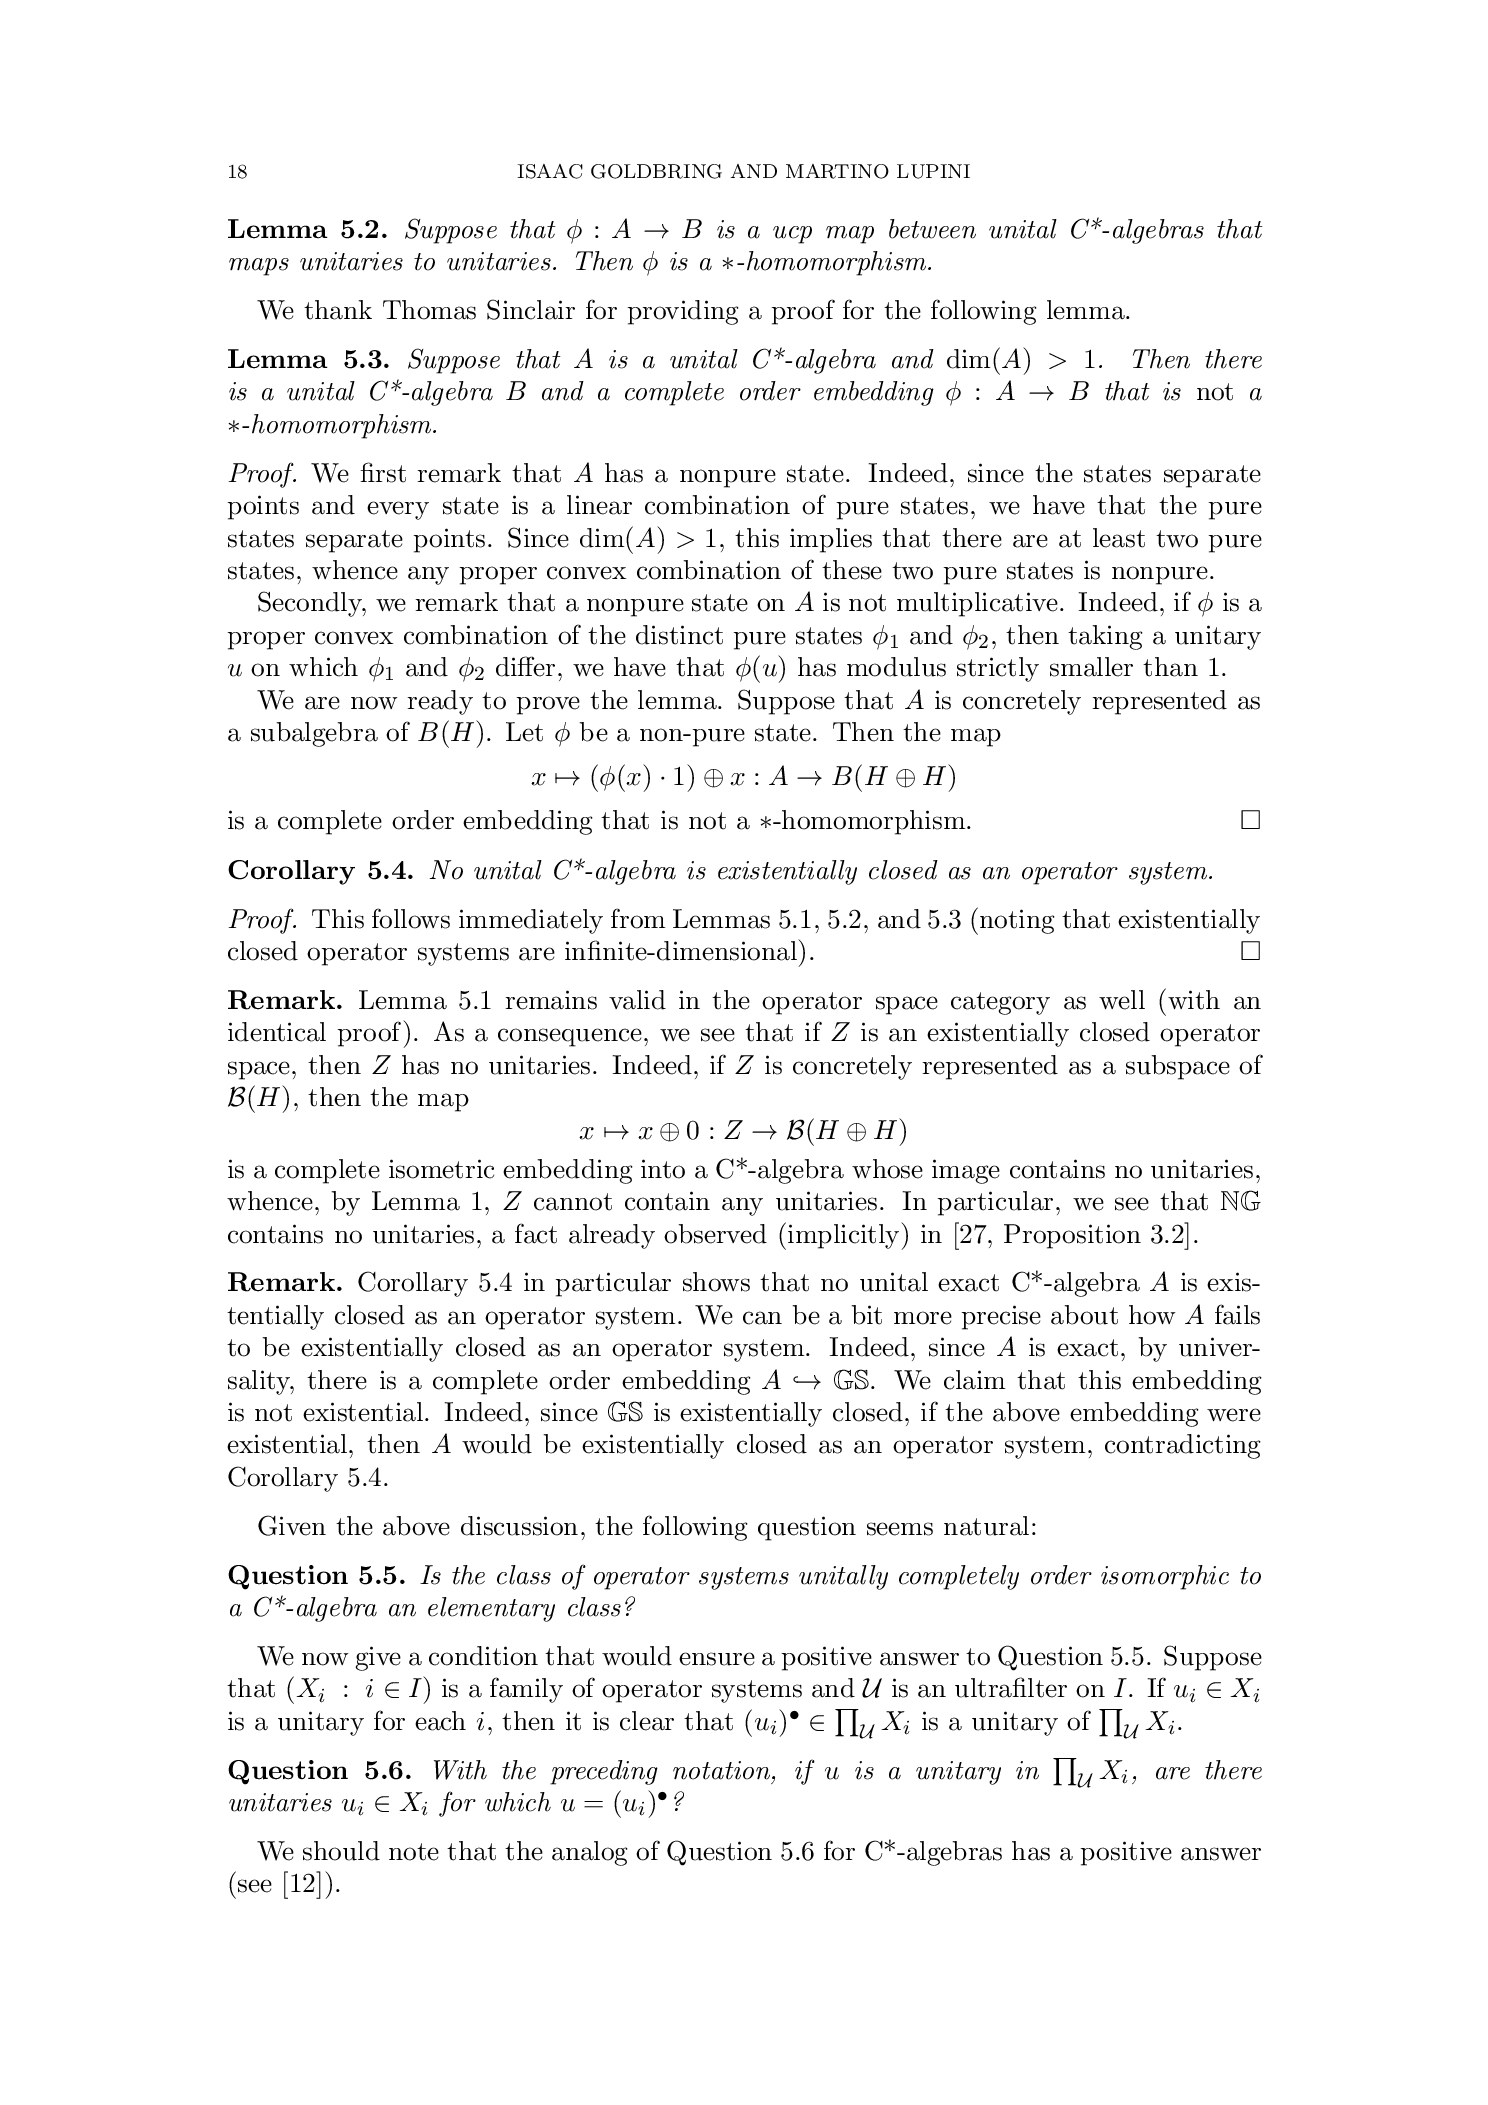
\includegraphics[width=0.78\textwidth]{figures/open_problem_page_18.png}
\end{center}

\section*{Result}

Question 5.6 has a negative answer.  The counterexample is a sequence of three-dimensional commutative operator systems.  Each factor contains no nonconstant unitaries, but the ultraproduct contains an element that is equal, in the ambient C*-ultraproduct, to the usual coordinate unitary \(z\in C(\T)\).

\section*{Proof Intuition}

The obstruction is non-stability of the metric equations defining unitaries in operator spaces.  Put
\[
f_\varepsilon(z)=z+\varepsilon z^2,\qquad 0<\varepsilon<1/4.
\]
Then \(f_\varepsilon\) is uniformly \(\varepsilon\)-close to the genuine unitary \(z\in C(\T)\).  Thus if \(\varepsilon_n\to0\), the element \((f_{\varepsilon_n})^\bullet\) becomes exactly unitary in the ambient C*-ultraproduct.

However, inside the small operator system
\[
X_\varepsilon=\operatorname{span}\{1,f_\varepsilon,\overline{f_\varepsilon}\}\subset C(\T),
\]
there is no nearby unitary.  The curve \(z+\varepsilon z^2\) is strictly convex, so the scalar part of the Blecher-Neal norm test forces any operator-space unitary in \(X_\varepsilon\) to have modulus one at every point of \(\T\).  A Laurent-polynomial calculation then says that the only such elements in \(X_\varepsilon\) are scalar constants.  These constants stay distance almost \(2\) from \(f_\varepsilon\), so they cannot lift the ultraproduct unitary.

\begin{lemma}[The factor unitaries are only constants]\label{lem:factor}
Let \(0<\varepsilon<1/4\), \(f_\varepsilon(z)=z+\varepsilon z^2\), and
\[
X_\varepsilon=\operatorname{span}\{1,f_\varepsilon,\overline{f_\varepsilon}\}\subset C(\T)
\]
with the inherited operator-space structure.  Then the unitaries of \(X_\varepsilon\) are exactly the scalar constants of modulus one.
\end{lemma}

\begin{proof}
Let \(v\in X_\varepsilon\) be a unitary in the operator-space sense.  We first prove that \(|v(\zeta)|=1\) for every \(\zeta\in\T\).

Consider the plane curve
\[
\gamma_\varepsilon(\theta)=e^{i\theta}+\varepsilon e^{2i\theta}.
\]
It is regular for \(\varepsilon<1/2\), and its signed curvature numerator is
\[
1+6\varepsilon\cos\theta+8\varepsilon^2.
\]
It is also injective: if \(z_1+\varepsilon z_1^2=z_2+\varepsilon z_2^2\), then
\[
(z_1-z_2)(1+\varepsilon(z_1+z_2))=0,
\]
and \(|\varepsilon(z_1+z_2)|\le 2\varepsilon<1\).  Thus \(z_1=z_2\).  For \(0<\varepsilon<1/4\) the curvature numerator is strictly positive for all \(\theta\), so \(\gamma_\varepsilon(\T)\) is a strictly convex Jordan curve.  In particular every point \(\gamma_\varepsilon(\theta_0)\) is strongly exposed by some real affine functional on \(\C\).

It follows that for every \(\zeta_0\in\T\) there is a self-adjoint element \(h\in X_\varepsilon\) whose absolute value has a unique maximum at \(\zeta_0\).  Indeed, take an exposing functional \(\ell(w)=\operatorname{Re}(\eta w)\) for \(w_0=f_\varepsilon(\zeta_0)\), and replace \(\ell(f_\varepsilon)\) by \(R+\ell(f_\varepsilon)\) with \(R\) large enough that the maximum of the absolute value is the unique positive maximum.

By the Blecher-Neal characterization of unitaries, applied only at matrix level \(1\) and to the row \([v\ h]\),
\[
\|[v\ h]\|^2=1+\|h\|^2.
\]
Since \(X_\varepsilon\subset C(\T)\), the left hand side is
\[
\sup_{\zeta\in\T}\left(|v(\zeta)|^2+|h(\zeta)|^2\right).
\]
As \(\|v\|=1\) and \(|h|\) has its unique maximum at \(\zeta_0\), this equality forces \(|v(\zeta_0)|=1\).  Since \(\zeta_0\) was arbitrary, \(|v|=1\) on \(\T\).

Now write
\[
v(z)=\alpha+\beta(z+\varepsilon z^2)+\gamma(z^{-1}+\varepsilon z^{-2}).
\]
Multiplying by \(z^2\) gives a polynomial
\[
q(z)=\gamma\varepsilon+\gamma z+\alpha z^2+\beta z^3+\beta\varepsilon z^4
\]
such that \(|q(z)|=1\) for every \(|z|=1\).  A polynomial with constant modulus one on \(\T\) is a scalar monomial \(c z^k\).  Comparing coefficients, the cases \(k=0,1,3,4\) are impossible because \(\varepsilon>0\) links adjacent nonzero coefficients.  The only possible case is \(k=2\), which gives \(\beta=\gamma=0\) and \(|\alpha|=1\).  Thus \(v\) is a scalar constant of modulus one.

The converse is immediate: scalar constants of modulus one are unitaries in \(X_\varepsilon\).
\end{proof}

\begin{theorem}[Negative answer to Question 5.6]\label{thm:counterexample}
Let \(\calU\) be any free ultrafilter on \(\mathbb N\).  There are operator systems \(X_n\) and a unitary \(u\in\prod_{\calU}X_n\) that cannot be represented as \(u=(u_n)^\bullet\) with each \(u_n\) a unitary of \(X_n\).
\end{theorem}

\begin{proof}
Set \(\varepsilon_n=1/(n+5)\), \(f_n(z)=z+\varepsilon_n z^2\), and
\[
X_n=\operatorname{span}\{1,f_n,\overline{f_n}\}\subset C(\T).
\]
Each \(X_n\) is a concrete unital self-adjoint subspace of \(C(\T)\), hence an operator system.  Let
\[
X=\prod_{\calU}X_n,\qquad A=\prod_{\calU} C(\T),
\]
and let \(j:X\to A\) be the natural complete isometric inclusion.  Put
\[
u=(f_n)^\bullet\in X,\qquad g=(z)^\bullet\in A.
\]
Since \(\|f_n-z\|=\varepsilon_n\to0\), we have \(j(u)=g\) in \(A\).  The element \(g\) is a unitary of the C*-algebra \(A\).  Therefore
\[
x\mapsto g^*j(x)
\]
is a linear complete isometry from \(X\) into \(A\) sending \(u\) to \(1_A\).  Thus \(u\) is a unitary of the operator space \(X\), hence a unitary in the sense of Question 5.6.

Suppose, toward a contradiction, that \(u=(u_n)^\bullet\) where each \(u_n\) is a unitary in \(X_n\).  By Lemma \ref{lem:factor}, \(u_n=\lambda_n1\) for some \(\lambda_n\in\T\).  For every \(\lambda\in\T\),
\[
\|f_n-\lambda\|_\infty
\ge |f_n(-\lambda)-\lambda|
=|-2\lambda+\varepsilon_n\lambda^2|
\ge 2-\varepsilon_n.
\]
Consequently,
\[
\|u-(u_n)^\bullet\|
=\lim_{\calU}\|f_n-\lambda_n\|_\infty
\ge \lim_{\calU}(2-\varepsilon_n)=2,
\]
contradicting \(u=(u_n)^\bullet\).  Hence no such unitary lift exists.
\end{proof}

\section*{Verification Notes}

The accompanying script \texttt{code/verify\_laurent\_curve\_checks.py} records the elementary scalar checks: the curvature lower bound \(1-6\varepsilon+8\varepsilon^2>0\) for the chosen range of \(\varepsilon\), the monomial coefficient alternatives, and the distance bound from \(f_\varepsilon\) to scalar unitaries.

The proof is not a counterexample to Question 5.5 itself.  It disproves the sufficient lifting condition proposed immediately after Question 5.5, namely Question 5.6.

\section*{Novelty and Literature Check}

Before promotion, the cheap run indexes were searched for arXiv:1501.04332 and the phrases ``Gurarij operator system'', ``unitarydefinable'', ``operator systems unitally completely order isomorphic'', and ``ultraproduct unitaries''.  No existing packet addressed Question 5.6.

External web search on 2026-07-18 used the exact label/text of Question 5.6 and close variants: ``unitarydefinable operator systems ultraproduct unitaries'', ``Is the class of operator systems unitally completely order isomorphic to a C*-algebra'', and ``unitaries operator systems ultraproduct Goldbring Lupini''.  The search located the source arXiv page and the Blecher-Neal characterization paper, but no later paper explicitly answering Question 5.6.

\section*{References}

\begin{thebibliography}{9}

\bibitem{GoldbringLupini}
I. Goldbring and M. Lupini,
\emph{Model-theoretic aspects of the Gurarij operator system},
arXiv:1501.04332v3, 2015.
\url{https://arxiv.org/abs/1501.04332}

\bibitem{BlecherNeal}
D. P. Blecher and M. Neal,
\emph{Metric characterizations of isometries and of unital operator spaces and systems},
Proceedings of the American Mathematical Society 139 (2011), 985--998;
arXiv:0805.2166.
\url{https://arxiv.org/abs/0805.2166}

\end{thebibliography}

\end{document}
